% V-model
\subsection{Approach}
This work has been implemented with an adaptation of V-model development process.
The original version of this process is known as a variation of the waterfall process,
with several phases dividing the beginning from the scratch and the final product,
but there is more emphasis on the coding phase.

A great feature of V-model is that every phase,
before the coding one,
has a 1:1 strong relationship with the phases that occurs after the coding,
reinforcing the mapping of the theoretical part of the project with the practical one.

The adaptation made in this project was to divide the V-model into iterations separated by the use cases.


\subsection{Use Cases}
\input{useCases/waterCycleControl}

\subsubsection{Summary table}

\begin{table}[h]
\centering
\caption{Requirements table}
\label{tab:requirementsTable}
\begin{tabular}{|c|c|c|}
\hline
\textbf{Use Case}    & \textbf{Requirement} & \textbf{Text} \\ \hline
Optimize Water Cycle & \ref{req1}           &                 \\ \hline
\end{tabular}
\end{table}

\subsection{Requirements}

\begin{description}

\item [\req{1}]
Optimize the water cycle period between fish tank and plants medium.

\end{description}

\subsection{System Design}

\begin{figure}[h]
    \centering
    \includegraphics[width=.8\linewidth]{diagrams/systemDesign}
    \caption{A simple diagram to represent a high level design of this project}
    \label{fig:highLevelSystemDesign}
\end{figure}

\subsection{System Architecture}

\begin{figure}[h]
    \centering
    \includegraphics[width=.8\linewidth]{diagrams/architecture_bb}
    \caption{This diagram shows how the microcontroller interacts with the water pump}
    \label{fig:waterCycleDiagram}
\end{figure}

\subsection{Prototype Implementation and Project Decisions}
There are a lot of authors that have had experience with Aquaponics automation.
Most of them chooses Arduino or Raspberry Pi as the main microcontroller.

Two great reasons for the Arduino's usage are:
This work's author already has an Arduino UNO,
but not a Raspberry PI.
Besides the main reference of this work,
the \cite{Kretzinger2015},
whose author has many years of experience with Aquaponics and its automation and he uses the Arduino as microcontroller.

The chosen components have been based in the references.

% Evaluation
% Related with the requirements:
% Test 1: R1: pH Control: change constant's value and verify control work
\subsection{Results and Evaluation}
